\documentclass[12pt,letterpaper]{article}
\usepackage[margin=1in]{geometry}
\usepackage{chngpage}
\usepackage[english]{babel}
\usepackage[utf8x]{inputenc}
\usepackage{amsmath}
\usepackage{amssymb} 
% \usepackage[retainorgcmds]{IEEEtrantools}
\usepackage{graphicx}
\usepackage{tabularx}
\usepackage{kpfonts}    % for nice fonts
\usepackage{microtype} 
\usepackage{booktabs}   % for nice tables
\usepackage{bm}         % for bold math
\usepackage{listings}   % for inserting code
\usepackage{verbatim}   % useful for program listings
\usepackage{color}  
\usepackage[colorlinks=true]{hyperref}
% use for hypertext
\hypersetup{
	colorlinks=false,       % false: boxed links; true: colored links
	linkcolor=green,        % color of internal links
	citecolor=blue,        % color of links to bibliography
	filecolor=magenta,     % color of file links
	urlcolor=blue         
}
\usepackage[colorinlistoftodos]{todonotes}
\usepackage{natbib}
\usepackage{float}
\usepackage{adjustbox}
\usepackage[capitalise]{cleveref}
\usepackage{xcolor}

\usepackage{longtable,threeparttablex}
\usepackage{subcaption}



%++++++++++++++++++++++++++++++++++++++++


\begin{document}

\begin{center}
\large IEMS-469 Dynamic Programming  HW4

\bigskip
Weijia Zhao \footnote{Weijia.Zhao@kellogg.northwestern.edu}\\
Kellogg Finance

\bigskip
This version: \today
\end{center}

\newpage



\section{Jester/UCB}
I set the weight of bonus to be  $\alpha=1$. I disable the update of parameters when use the model in "testing" mode (i.e. this is different from online learning, when we are given new samples one by one and update the parameters in the meantime. In my analysis, the actual reward can only be observed altogether in the end when doing evaluation).\\
 
Seems to me that we can choose to go over the training sample multiple times but the improvement of performance is not very significant. In general, the cumulative reward is very close to a linear function of the number of observations in testing set. The total regret for 1200 observations is about 3000 (I did several experiments and the highest I got is 3091 and the lowest I got is 3007)

 \begin{figure}[H]
	\centering
	\caption{Jester}
		\centering
		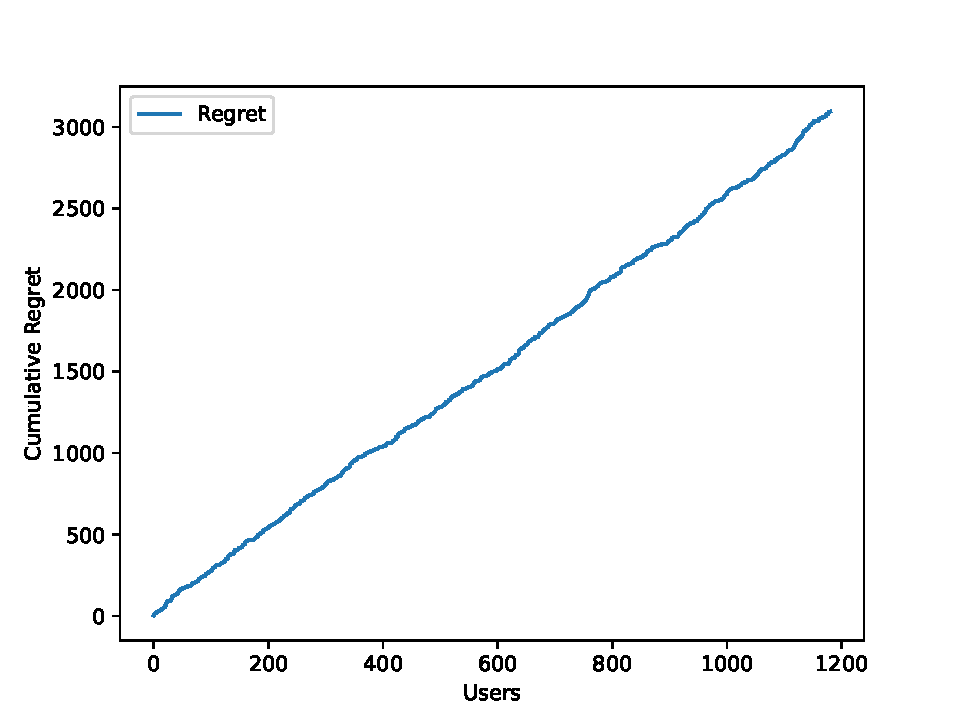
\includegraphics[width=\textwidth]{/Users/lesliezhao/Dropbox/nu_course/2021_fall/DP/IEMS469_HW_LWZ/hw4/results.pdf}
\end{figure}



\end{document}
